\clearpage
\section{Sacred Vessels and Altar Linens}
\PCDPlateHeader{Plate III --- Sacred Vessels and Vessels for Communion}{Not to common scale}
\ifdefined\TriptychPrintEdition
\begin{center}
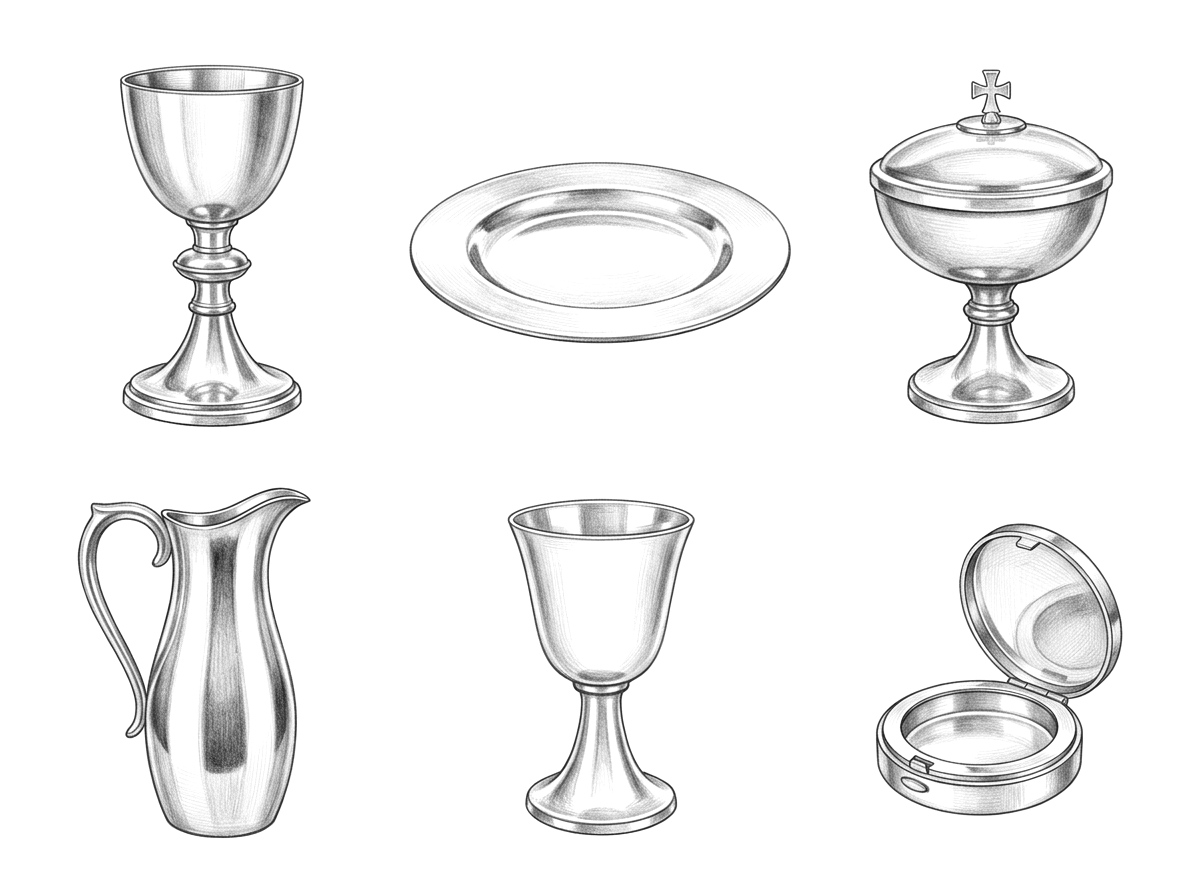
\includegraphics[width=0.92\linewidth,height=3.55in,keepaspectratio]{liturgy/roman-rite/postconciliar/2008-latin-2011-us-english/reference/roman-sanctuary-dictionary/shared/artwork/graphite/pc-art-03-sacred-vessels.png}
\end{center}
\PCDPositionKey{Top row, left to right: Chalice, wide shallow Paten, lidded footed Ciborium with cross finial. Bottom row, left to right: pitcher-style wine Flagon (pre-consecration transport only), footed Communion Cup (chalice), hinged pocket Pyx shown open.}
\else
\textbf{Visual Plate Summary (Plate III --- Sacred Vessels and Vessels for Communion, Not to common scale):} Six-vessel monochrome graphite comparison rendered with metallic reflections on white ground: top row left to right, a classical footed chalice with node, a broad shallow paten dish, and a lidded footed ciborium topped by a small cross; bottom row left to right, a tall slender pitcher-style wine flagon for bringing unconsecrated wine, a simpler footed Communion cup for distributing the Precious Blood, and a small hinged circular pocket pyx open to show its smooth gilded cavity.

\textbf{Reading order and object placement:} Top row, left to right: Chalice, wide shallow Paten, lidded footed Ciborium with cross finial. Bottom row, left to right: pitcher-style wine Flagon (pre-consecration transport only), footed Communion Cup (chalice), hinged pocket Pyx shown open.
\fi

\label{pc-obj-chalice}
\PCDEntryHead{Chalice}{Calix}{required}{N08}
\PCDField{Also called}{Principal Chalice; Eucharistic Chalice; \textit{Calix principalis}}
Among all sacred vessels in the sanctuary, the chalice receives foremost honor because it holds the Precious Blood of Christ offered on the altar (GIRM 327). Shaped with a deep cup, a central node for secure lifting, and a stable base, it stands quietly on the credence table during the Liturgy of the Word and comes to the center of the altar for the Eucharistic sacrifice.

\PCDField{On the plate}{Top left (Plate III); center of the unfolded corporal (Plate X)}
\PCDField{Symbolism}{The chalice bears singular honor as the cup of the New Covenant, recalling the Lord's words at the Last Supper in Matt 26:27--28 (``Drink ye all of this. For this is my blood of the new testament, which shall be shed for many unto remission of sins.''), St. Paul in 1 Cor 10:16 (``The chalice of benediction which we bless, is it not the communion of the blood of Christ?''), and Ps 115:13 [Heb 116:13] (``I will take the chalice of salvation; and I will call upon the name of the Lord.''). St. Thomas Aquinas teaches that the chalice signifies both the Passion of Christ and the joy of the blessed, and explains that non-porous precious metal---rather than wood, stone, or glass---is required out of reverence for Christ's Blood. (GIRM 327; Matt 26:27--28; 1 Cor 10:16; Ps 115:13 [Heb 116:13]; St. Thomas Aquinas, Summa Theologiae III, q. 83, a. 3, ad 6 \& a. 5, ad 9)}
\PCDField{Relation to the 1962 Missal}{\PCDTag{materially changed} Whereas the 1962 Roman Missal required a gold or silver-cupped chalice consecrated with Sacred Chrism by a bishop and carried into Low Mass veiled with a stiff burse by the priest himself (RS I.1, II.1), the 2008/2011 Missal appoints a liturgical blessing by bishop or priest (GIRM 333), ordinarily prepares the chalice on the credence table until the Preparation of the Gifts (GIRM 118c, 139), and commends the chalice veil as a praiseworthy optional practice while leaving the burse unnamed.}
\PCDEntryRule

\label{pc-obj-paten}
\PCDEntryHead{Paten}{Patena}{required}{N09}
\PCDField{Also called}{Eucharistic Paten; Large Paten; \textit{Patena maior}}
The shallow circular dish that rests beside the chalice holds the bread that becomes the Body of Christ. While earlier practice used a small disc sized for the priest's host alone, the postconciliar Roman Missal encourages a broader paten able to hold the bread for priest, ministers, and faithful together, giving visible expression to St. Paul's teaching that many share one bread (GIRM 331; 1 Cor 10:17).

\PCDField{On the plate}{Top center (Plate III); front center of the unfolded corporal (Plate X)}
\PCDField{Symbolism}{Together with the chalice, the paten receives special honor as the receptacle of the Eucharistic Bread (GIRM 327). A larger paten holding hosts for priest, deacon, ministers, and assembly visibly expresses 1 Cor 10:17 (``For we, being many, are one bread, one body: all that partake of one bread.''). St. Thomas Aquinas pairs the paten with the chalice as a figure of the tomb that held the Lord's Body, grounding the demand for noble, unbreakable material in reverence for Christ. (GIRM 327, 331; 1 Cor 10:17; St. Thomas Aquinas, Summa Theologiae III, q. 83, a. 3, obj. 6 \& ad 6)}
\PCDField{Relation to the 1962 Missal}{\PCDTag{materially changed} In the 1962 Roman Missal, the paten was a small flat gilded metal disc consecrated by a bishop, sized for the celebrant's single host, kissed and used to sign the celebrant at the Libera nos, and held veiled by the subdeacon at Solemn Mass (RS I.1, VII.9, X.1--2). The 2008/2011 GIRM omits the signing and kissing at the Libera nos, introduces a broad paten fittingly holding hosts for clergy and faithful alike (GIRM 331), and under USCCB GIRM 329 admits solid noble non-metal materials.}
\PCDEntryRule

\label{pc-obj-ciborium}
\PCDEntryHead{Ciborium}{Pyxis}{provided}{N10}
\PCDField{Also called}{Host Vessel; Covered Ciborium; \textit{Ciborium}; \textit{Vas}}
Shaped like a broad footed cup with a cross-topped lid, the ciborium holds the consecrated Hosts during distribution of Holy Communion and safeguards the Blessed Sacrament inside the tabernacle for the sick and for adoration. While the Latin Missal continues to call it by the ancient word pyxis, English usage distinguishes the larger altar ciborium from the small pocket pyx carried to the homebound.

\PCDField{On the plate}{Top right (Plate III); draped in a white veil at rear right of the corporal (Plate X)}
\PCDField{Relation to the 1962 Missal}{\PCDTag{continued} Both the 1962 Roman Missal (using Latin pyxis or vas) and the 2008/2011 IGMR (continuing Latin pyxis, rendered ``ciborium'' in English) appoint a blessed covered vessel for consecrating, distributing, and reserving the Sacred Hosts. Postconciliar norms expand distribution use to broad dignified bowls alongside stemmed ciboria, admit approved non-metal solid noble materials in the United States (US GIRM 329), and treat the silk ciborium veil as customary rather than universally mandated.}
\PCDEntryRule

\label{pc-obj-pyx}
\PCDEntryHead{Pyx}{Pyxis parva}{provided}{N11}
\PCDField{Also called}{Sick-Call Pyx; Pocket Pyx; \textit{Theca}; \textit{Pyxis}}
Barely wider than a pocket watch, the hinged metal pyx enables the Church to carry Christ's Eucharistic presence beyond the church doors to hospital beds and homebound parishioners---especially as Viaticum, food for the journey, for the dying. St. Thomas Aquinas notes that the Church reserves consecrated hosts above all so the sick may never lack the sacrament in danger of death (Summa Theologiae III, q. 83, a. 5, ad 11).

\PCDField{On the plate}{Bottom right, shown hinged open to display the recessed interior (Plate III)}
\PCDField{Relation to the 1962 Missal}{\PCDTag{continued} The portable hinged metal pyx carried in a pouch for Communion of the sick continues unchanged in construction from the 1962 Roman Ritual (Title IV, ch. 2) into postconciliar discipline (GIRM 329; CIC can. 939). Postconciliar pastoral law narrows English usage of ``pyx'' specifically to this portable sick-call container and extends its authorized pastoral carriage to formally deputed extraordinary ministers alongside clergy.}
\PCDEntryRule

\label{pc-obj-communion-cup}
\PCDEntryHead{Communion Cup}{Calix}{territorial adaptation}{N12}
\PCDField{Also called}{Communion Chalice; Additional Chalice; \textit{Calix ad Communionem sub utraque specie}}
Because the postconciliar Roman Rite restored Communion under both kinds to the lay faithful, parishes regularly place additional chalices---commonly called Communion cups---beside the main chalice on the altar. Each cup meets the same sacred-vessel standard as the principal chalice, is filled before the consecration, and is paired with a white purificator so the rim is wiped reverently for every communicant (GIRM 285--286; USCCB Norms 32--36).

\PCDField{On the plate}{Bottom center (Plate III); flanking the principal chalice beside folded purificators (Plate X)}
\PCDField{Symbolism}{Holy Communion takes on a fuller form as a sign when received under both kinds, manifesting more clearly the Eucharistic banquet and the new and eternal Covenant ratified in Christ's Blood (GIRM 281; USCCB Norms 32--33). It echoes 1 Cor 11:25--26 (``This chalice is the new testament in my blood. This do ye, as often as you shall drink, for the commemoration of me.'') and Matt 26:27--28 (``Drink ye all of this.''). (GIRM 281; USCCB Norms for Holy Communion under Both Kinds (2011) 32--33; Matt 26:27--28; 1 Cor 10:16; 1 Cor 11:25--26)}
\PCDField{Relation to the 1962 Missal}{\PCDTag{newly provided} In the 1962 Roman Missal, lay faithful received Holy Communion exclusively under the species of bread (RG 503; RS X.6), so no supplementary Communion chalices existed. Following Sacrosanctum Concilium 55, GIRM 281--287 and the USCCB Norms newly provide for additional chalices governed by the full sacred-vessel standards of GIRM 328--330.}
\PCDEntryRule

\label{pc-obj-cruets}
\PCDEntryHead{Cruets}{Urceoli}{required}{N13}
\PCDField{Also called}{Wine and Water Cruets; \textit{Ampullae}; \textit{Urceoli cum vino et aqua}}
Resting quietly on the side credence table, the small pair of wine and water cruets supplies the unconsecrated wine that becomes Christ's Blood and the water mingled into it before the Eucharistic Prayer---as well as the water used afterward to purify the sacred vessels. Clear glass has long been preferred so the server and priest can distinguish wine from water immediately.

\PCDField{On the plate}{See Plate VI, top left (paired with stoppers on an oval metal tray); Plate I, atop the credence table}
\PCDField{Relation to the 1962 Missal}{\PCDTag{continued} Both the 1962 Roman Missal (using Latin ampullae, RG 528) and the 2008/2011 IGMR (using Latin urceoli, GIRM 118c) appoint paired wine and water cruets on the credence table for the Offertory mixing and ablutions. Postconciliar rubrics omit kissing the cruets and signing the water cruet with the cross, and allow the wine to be carried from the nave in the Procession of the Gifts (GIRM 140).}
\PCDEntryRule

\label{pc-obj-flagon}
\PCDEntryHead{Flagon}{Lagoena}{permitted}{N14}
\PCDField{Also called}{Wine Pitcher; Offertory Carafe; \textit{Lagena}; \textit{Ampulla maior}}
Because larger Sunday congregations often receive Holy Communion from several chalices, parishes frequently use a tall pitcher called a flagon to carry the unconsecrated wine forward in the Procession of the Gifts. Church law draws a sharp line here: the flagon serves solely to bring wine to the altar before the Eucharistic Prayer, where it is poured into true chalices; it is never left on the altar to hold or pour the consecrated Blood of Christ (Redemptionis Sacramentum 106).

\PCDField{On the plate}{Bottom left, tall slender pitcher with curved handle and pouring lip (Plate III)}
\PCDField{Relation to the 1962 Missal}{\PCDTag{no established counterpart} The 1962 Roman Missal had no counterpart to a wine flagon because lay Communion was distributed under the species of bread alone and small cruets on the credence table sufficed (RG 528). The flagon emerged with the postconciliar gifts procession and Communion under both kinds, and was strictly restricted to pre-consecration wine transport by Redemptionis Sacramentum 106 (2004).}
\PCDEntryRule

\clearpage
\PCDPlateHeader{Plate IV --- Altar and Vessel Linens}{Not to common scale}
\ifdefined\TriptychPrintEdition
\begin{center}
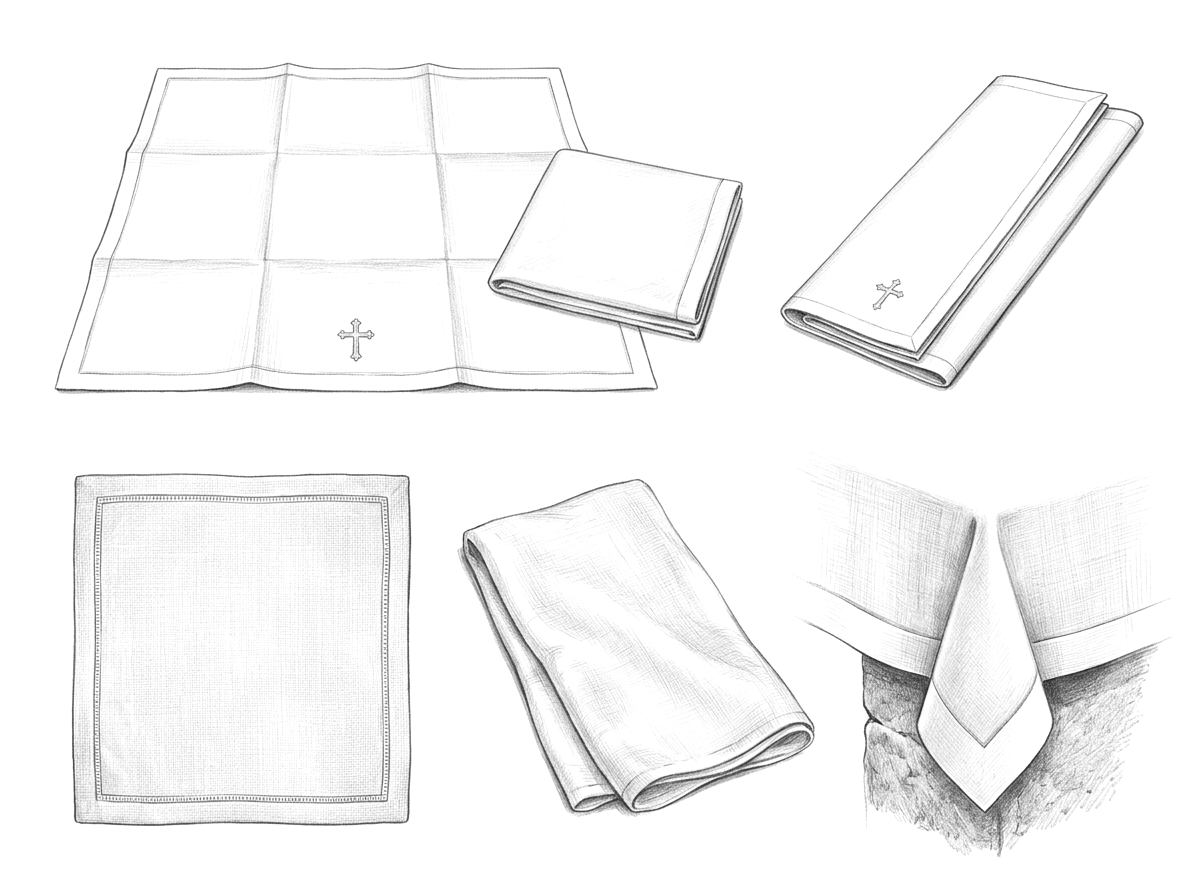
\includegraphics[width=0.92\linewidth,height=3.55in,keepaspectratio]{liturgy/roman-rite/postconciliar/2008-latin-2011-us-english/reference/roman-sanctuary-dictionary/shared/artwork/graphite/pc-art-04-white-linens.png}
\end{center}
\PCDPositionKey{Top left: unfolded square Corporal showing its three-by-three fold grid and front stitched cross, paired with a folded Corporal; top right: oblong Purificator folded lengthwise in thirds with stitched cross visible near the lower folded end; bottom left: stiffened square Pall; bottom center: folded Lavabo Towel; bottom right: hemmed corner of white Altar Cloth draped over the mensa.}
\else
\textbf{Visual Plate Summary (Plate IV --- Altar and Vessel Linens, Not to common scale):} Five-subject monochrome graphite textile study on pure white stock differentiating white altar linens by crease geometry and drape: top left, an unfolded square corporal creased into nine squares with a small stitched cross near the front center edge beside a folded square corporal; top right, an oblong purificator folded lengthwise in thirds with a small stitched cross visible near the lower folded end; bottom left, a rigid flat square linen pall; bottom center, a softly folded rectangular lavabo finger towel; bottom right, a hemmed corner of a white altar cloth hanging over a stone altar edge.

\textbf{Reading order and object placement:} Top left: unfolded square Corporal showing its three-by-three fold grid and front stitched cross, paired with a folded Corporal; top right: oblong Purificator folded lengthwise in thirds with stitched cross visible near the lower folded end; bottom left: stiffened square Pall; bottom center: folded Lavabo Towel; bottom right: hemmed corner of white Altar Cloth draped over the mensa.
\fi

\label{pc-obj-altar-cloth}
\PCDEntryHead{Altar Cloth}{Mappa}{required}{N15}
\PCDField{Also called}{Fair linen; Altar linen; \textit{Mappa altaris}; \textit{Mappae}; \textit{Tobalea}}
Before Mass begins, the bare stone or wood altar is vested in clean white linen. The Church prescribes at least one white altar cloth out of reverence for the memorial of Christ's sacrifice and the Eucharistic banquet offered upon the mensa (GIRM 117, 304). In the United States, parishes may layer additional cloths of festive Christian colors underneath, while always keeping white as the uppermost cloth.

\PCDField{On the plate}{Bottom right corner drape (Plate IV); dressing the altar (Plates I--II)}
\PCDField{Symbolism}{The white altar cloth expresses reverence for the celebration of the Lord's memorial and the sacred banquet in which his Body and Blood are offered. In the scholastic tradition of St. Thomas Aquinas, the clean linen dressing the altar also evokes the burial cloth of Christ---``And Joseph taking the body wrapped it up in a clean linen cloth'' (Matt 27:59)---calling to mind purity of conscience and the Passion of the Lord. (GIRM 304; St. Thomas Aquinas, Summa Theologiae III, q. 83, a. 3, ad 7; Matt 27:59)}
\PCDField{Relation to the 1962 Missal}{\PCDTag{materially changed} The 1962 Roman Missal required three clean blessed white linen cloths covering the altar, with the uppermost cloth reaching the ground at both sides (RG 526). Postconciliar law requires at least one white cloth suited to the altar's shape and size (GIRM 117, 304), while the United States adaptation permits additional festive colored under-cloths beneath the white top cloth.}
\PCDEntryRule

\label{pc-obj-corporal}
\PCDEntryHead{Corporal}{Corporale}{required}{N16}
\PCDField{Also called}{Altar corporal; \textit{Palla corporalis}}
Named from the Latin word corpus (``body''), this square of crisp white linen lies directly beneath the chalice, paten, and ciboria during the Eucharistic Prayer and Communion. Unfolded at the Preparation of the Gifts and folded inward afterward, it safeguards even the tiniest particle of the Sacred Host and recalls the clean linen shroud of Christ's burial.

\PCDField{On the plate}{Top left, shown unfolded in a 3x3 crease grid and folded beside it (Plate IV); beneath vessels (Plate X)}
\PCDField{Symbolism}{Named from the Latin corpus (``body''), the corporal is made of pure white linen because Christ's body was wrapped in a clean linen shroud at his burial: ``And Joseph taking the body wrapped it up in a clean linen cloth'' (Matt 27:59; cf. John 20:6, ``and saw the linen cloths lying''). Following ancient Roman tradition expounded by St. Thomas Aquinas, the white linen signifies purity of conscience and recalls the Passion of Christ. (St. Thomas Aquinas, Summa Theologiae III, q. 83, a. 3, ad 7 (citing De Consecr. dist. 1); Matt 27:59; John 20:6)}
\PCDField{Relation to the 1962 Missal}{\PCDTag{continued} The square white linen corporal folded inward in nine squares continues directly from the 1962 Roman Missal (RS I.1). In postconciliar Mass with a congregation, it is placed on the altar at the Preparation of the Gifts rather than drawn from a stiff burse at the start of Low Mass (1962 RS II.2), and GIRM 118c no longer mandates a burse.}
\PCDEntryRule

\label{pc-obj-purificator}
\PCDEntryHead{Purificator}{Purificatorium}{required}{N17}
\PCDField{Also called}{Chalice cloth}
This narrow folded strip of absorbent white linen accompanies every chalice at Mass. During Communion under both kinds, ministers carefully wipe the chalice rim with a clean fold after each communicant; afterward, the priest, deacon, or instituted acolyte uses it to dry the sacred vessels once they have been purified. Because it comes into direct contact with the Precious Blood, the Church mandates reverent hand-rinsing into the sacrarium before regular laundering.

\PCDField{On the plate}{Top right, folded lengthwise in thirds with stitched cross visible near the lower folded end (Plate IV); beside Communion cups (Plate X)}
\PCDField{Relation to the 1962 Missal}{\PCDTag{continued} The folded white linen purificator continues directly from the 1962 Roman Missal (RS I.1, X.5), where a single purificator served the celebrant's chalice and ablutions. In postconciliar celebration, Communion under both kinds expands its use so that a separate clean purificator accompanies every Communion chalice (GIRM 286).}
\PCDEntryRule

\label{pc-obj-pall}
\PCDEntryHead{Pall}{Palla}{optional}{N18}
\PCDField{Also called}{Chalice pall; \textit{Palla calicis}}
This crisp, stiffened white square rests flat across the top of the chalice like a clean linen lid. Serving a practical office of reverence, it protects the wine and the Precious Blood from dust or insects, and postconciliar rubrics make its use optional whenever pastoral conditions call for it (GIRM 118c).

\PCDField{On the plate}{Bottom left, stiffened square (Plate IV)}
\PCDField{Relation to the 1962 Missal}{\PCDTag{optional} The 1962 Roman Missal required a blessed small linen pall on every prepared chalice stack to cover the host and chalice throughout the Offertory and Canon (RS I.1, VII.5, VIII.7). Postconciliar law expressly makes the pall optional, prescribing it ``if appropriate'' (pro opportunitate, GIRM 118c).}
\PCDEntryRule

\label{pc-obj-lavabo-towel}
\PCDEntryHead{Lavabo Towel}{Manutergium}{required}{N19}
\PCDField{Also called}{Finger towel; Hand towel; \textit{Tersorium}}
After the bread and wine are set upon the altar (and after the incensation when incense is used), a server brings water, a shallow basin, and this plain white hand towel to the side of the altar. While the towel itself serves a purely practical purpose, the handwashing action it supports expresses the priest's desire for interior purification before the Eucharistic Prayer (GIRM 76), echoing the psalmist's prayer: ``Wash me yet more from my iniquity, and cleanse me from my sin'' (Ps 50:4 [51:2]).

\PCDField{On the plate}{Bottom center, softly folded rectangular cloth (Plate IV); paired with lavabo pitcher and basin (Plate VI)}
\PCDField{Relation to the 1962 Missal}{\PCDTag{continued} The hand towel (manutergium) prepared with water and basin on the credence table continues directly from the 1962 Roman Missal (RG 528; RS VII.6--7, VII.10). In the postconciliar rite, the priest washes his hands rather than only thumb and forefinger tips, and replaces Psalm 25:6--12 (Lavabo inter innocentes) with the single verse of Psalm 50:4 [51:2] praying for interior cleansing (GIRM 76, 145).}
\PCDEntryRule
